
\documentclass[]{report}
%% PACKAGES
\usepackage{graphicx}
\usepackage{listings,amsmath}
\usepackage{microtype,todonotes}

%% GRAPHICS RELATED
\usepackage[outdir=./tmp/]{epstopdf}
\graphicspath{{../images/}{./tmp}}
\DeclareGraphicsExtensions{.eps, .pdf, .jpeg, .png}

%% BIBLIOGRAPHY
\bibliographystyle{ieeetr}

%% CPATION SETUP
\usepackage{caption}
\usepackage{subcaption}
\usepackage{subfig}
\captionsetup{belowskip=12pt,aboveskip=4pt}

%% USER COMMANDS
\newcommand{\iso}[2]{${}^{#2}${#1}}

\title{Energy Deposition in Polymers}
\author{Matthew J. Urffer}
\date{\today}

\begin{document}

% Cover Page
\maketitle

% To Do List
\listoftodos

\section{Introduction}

A supervised machine learning problem is one which a learning algorithm is presented a set of training data and attempts to find an unknown function which maps the training values to the correct answer.
Typically the training set, denoted $S$, is a set of the form $\left \{ (\vec{x}_1,y_1), (\vec{x}_2,y_2), \dots, (\vec{x}_n,y_n) \right \}$ where $\vec{x}_i$ is vector of some features of the problem.
Examples of problem features include discrete or real valued items such as height, weight, age, zip code, grade point average, starting salary, and telephone number (as just a few)  which might make up the features of a person.
The $y_i$ are the class of the training feature $\vec{x}_i$ belongs to; these might be University of Tennessee students or Carnegie Mellon students.
In this examples students with a zip code of 15213 are likely to be Tartans, while students with a zip code of 37916 are like to be Volunteers.
The challenge arises from examples have overlapping features; for example this author as a former Tartan and current Vol would be difficult to classify by zip code.
The learning algorithms job is then to find a hypothesis $h$ that correctly classifies a student as a Volunteer of Tartan based on the features provided.
This learning process can then be defined as finding the hypothesis that has the least error (incorrect classifications) on the training data set while extending to examples outside of the training space.

\subsection{Support Vector Machines}
Support Vector Machines (SVM) are a supervised learning technique in which hyperplanes are constructed in a high dimensional space to which the features are mapped.
SVMs find the hyperplanes that are the farthest away from all of mapped features in order to provide excellent training performance while still maintaining the ability to generalize to new instances; i.e. SVMs are maximal margin classifiers.
For a binary classification the decision function of the SVM is the dot product of the weight vector and the training example in the feature space added to a bias vector as shown in Equation \ref{eq:BCSVM}.
\begin{equation}
\label{eq:BCSVM}
f \left ( \vec{x} \right ) = \left \langle \vec{w} \phi(\vec{x}) \right \rangle + \vec{b}
\end{equation}
where $\phi(\vec{x})$ is a mapping to the higher dimensional space.
The SVM is then learning the optimal values of the weight vector $\vec{w}$ and the basis $\vec{b}$.

The radial basis function (Equation \ref{eq:RBF}) is a common kernel function used to map the input vector $\vec{x}$ into a higher dimension.
\begin{equation}
\label{eq:RBF}
k \left ( \vec{x}_i , \vec{x}_j \right ) = exp \left ( - \frac{\left \| \vec{x}_i - \vec{x}_j \right \|}{2\sigma^2} \right ) 
\end{equation}
The maximal margin is ensured by minimizing:
\begin{equation}
\label{eq:Min}
g(\vec{w},\eta) = \frac{1}{2} \left \| \vec{w} \right \| + C \sum_{i=1}^N \zeta_i
\end{equation}
subject to:
\begin{equation}
\label{eq:Constraint}
y_i( \left \langle \vec{w},\phi(\vec{x}) \right \rangle + b ) \ge 1-\zeta_i, ~~~\zeta_i \ge 0
\end{equation}
where $\zeta_i$ is the $i$th slack variable and C is the regularization parameter \cite{li_adaboost_2008}.
This problem can be translated  in to the Wolfe dual form, which can be solved with quadratic programing \cite{li_adaboost_2008}.

\subsection{Boosting}
Unbalanced data sets (data sets in which a majority of the values come from one class, see Figure \ref{fig:ClassDist}) are difficult for classification schemes to learn because the minority class is not well represented and tends to be thought as noise for the classifier.
Often classifiers are trained from unbalanced data sets by artificially balancing the data set by sampling techniques; i.e. up-sampling (sampling more from the minority class) and down-sampling (sampling less from the majority class).
Boosting is an ensemble learning method in which a set of weights is maintained over the training samples and adaptively adjusted after each training iteration according to the ones that are misclassified \cite{li_adaboost_2008}.
Given an individual classifier $h$, an ensemble of classifiers can be constructed of a set of individual classifiers, $H={h_1, h_2,\dot, h_n}$.
By maintaining a weight distribution over all of the training examples, these weights could be updated to emphasize the training examples that are misclassified incorrectly.  These incorrectly classified examples could then be learned in a refinement of the classifier or by training adding a new classifier to the ensemble with the new weights.
Performance of the ensemble is enhanced as long as the individual classifiers are weak and have uncorrelated errors as when any single classifier is incorrect the other classifiers in the ensemble might correctly classify the example.
\begin{figure*}[ht!]
	\centering
	\begin{subfigure}[b]{0.3\textwidth}
		\centering
		\includegraphics[width=\textwidth]{Liver_ClassDist}
        \caption{Liver}
	\end{subfigure}%
	~
	\begin{subfigure}[b]{0.3\textwidth}
		\centering
		\includegraphics[width=\textwidth]{Glass_ClassDist}
        \caption{Glass}
	\end{subfigure}	
    ~
	\begin{subfigure}[b]{0.3\textwidth}
		\centering
		\includegraphics[width=\textwidth]{Vowel_ClassDist}
        \caption{Vowel}
	\end{subfigure}%
	\caption{Distribution of Class Data}
	\label{fig:ClassDist}
\end{figure*}

This document is organzied as follows.
A brief overview of the interaction of charged particles in matter will be provided in Section \ref{sec:PreviousWork}, as well as some prelimary experiments demonstrating the range of secondary electrons to aid in neutron-gamma discrimination.
Next, the use of the GEANT4 toolkit for the modeling of the energy depostion will be discussed, as well as the validation of the model in Section \ref{sec:Methods}.
In the \ref{sec:Results} the results of this model applied to a single film will demonstrate the enhanced ability of neutron-gamma discrimination through secondary electrons.

%%%%%%%%%%%%%%%%%%%%%%%%%%%%%%%%%%%%%%%%%%%%%

\section{Previous Work}
\label{sec:PreviousWork}
Previous work on the energy deposition of thin focused on spectra measurements from fabricated films as wells as single collision energy loss spectra.
A sequence of 10\% \iso{Li}{6}F, 5\% PPOPOPOP films in a PS matrix cast to thickness between 15 and 600 $\mu$m where fabricated and the response was measured from a gamma source as well as a neutron source.
These experiment results are shown in \ref{sec:SpectraMeasurements}.


\subsection{Spectra Measurements}
\label{sec:SpectraMeasurements}
Evidence that the secondary electrons contribute to energy loss can be seen in Figure \ref{fig:SpectraFeatures} where there is an increase in the endpoint of the spectra as films become thicker.
This increase in the spectra endpoint is indicative of the film producing more light, and as the light collection geometry remained constant the increase in the endpoint is attributed to a larger energy deposition in the 50 $\mu$m film compared to the 15 $\mu$m or 25 $\mu$m film.
%%%%%%%%%%%%%%%%%%%% Figures %%%%%%%%%%%%%%%%%%%%%%%%
\begin{figure}
    \centering
    \caption{Spectra properties as a function of film thickness}
    \begin{subfigure}[b]{0.45\figurewidth}
        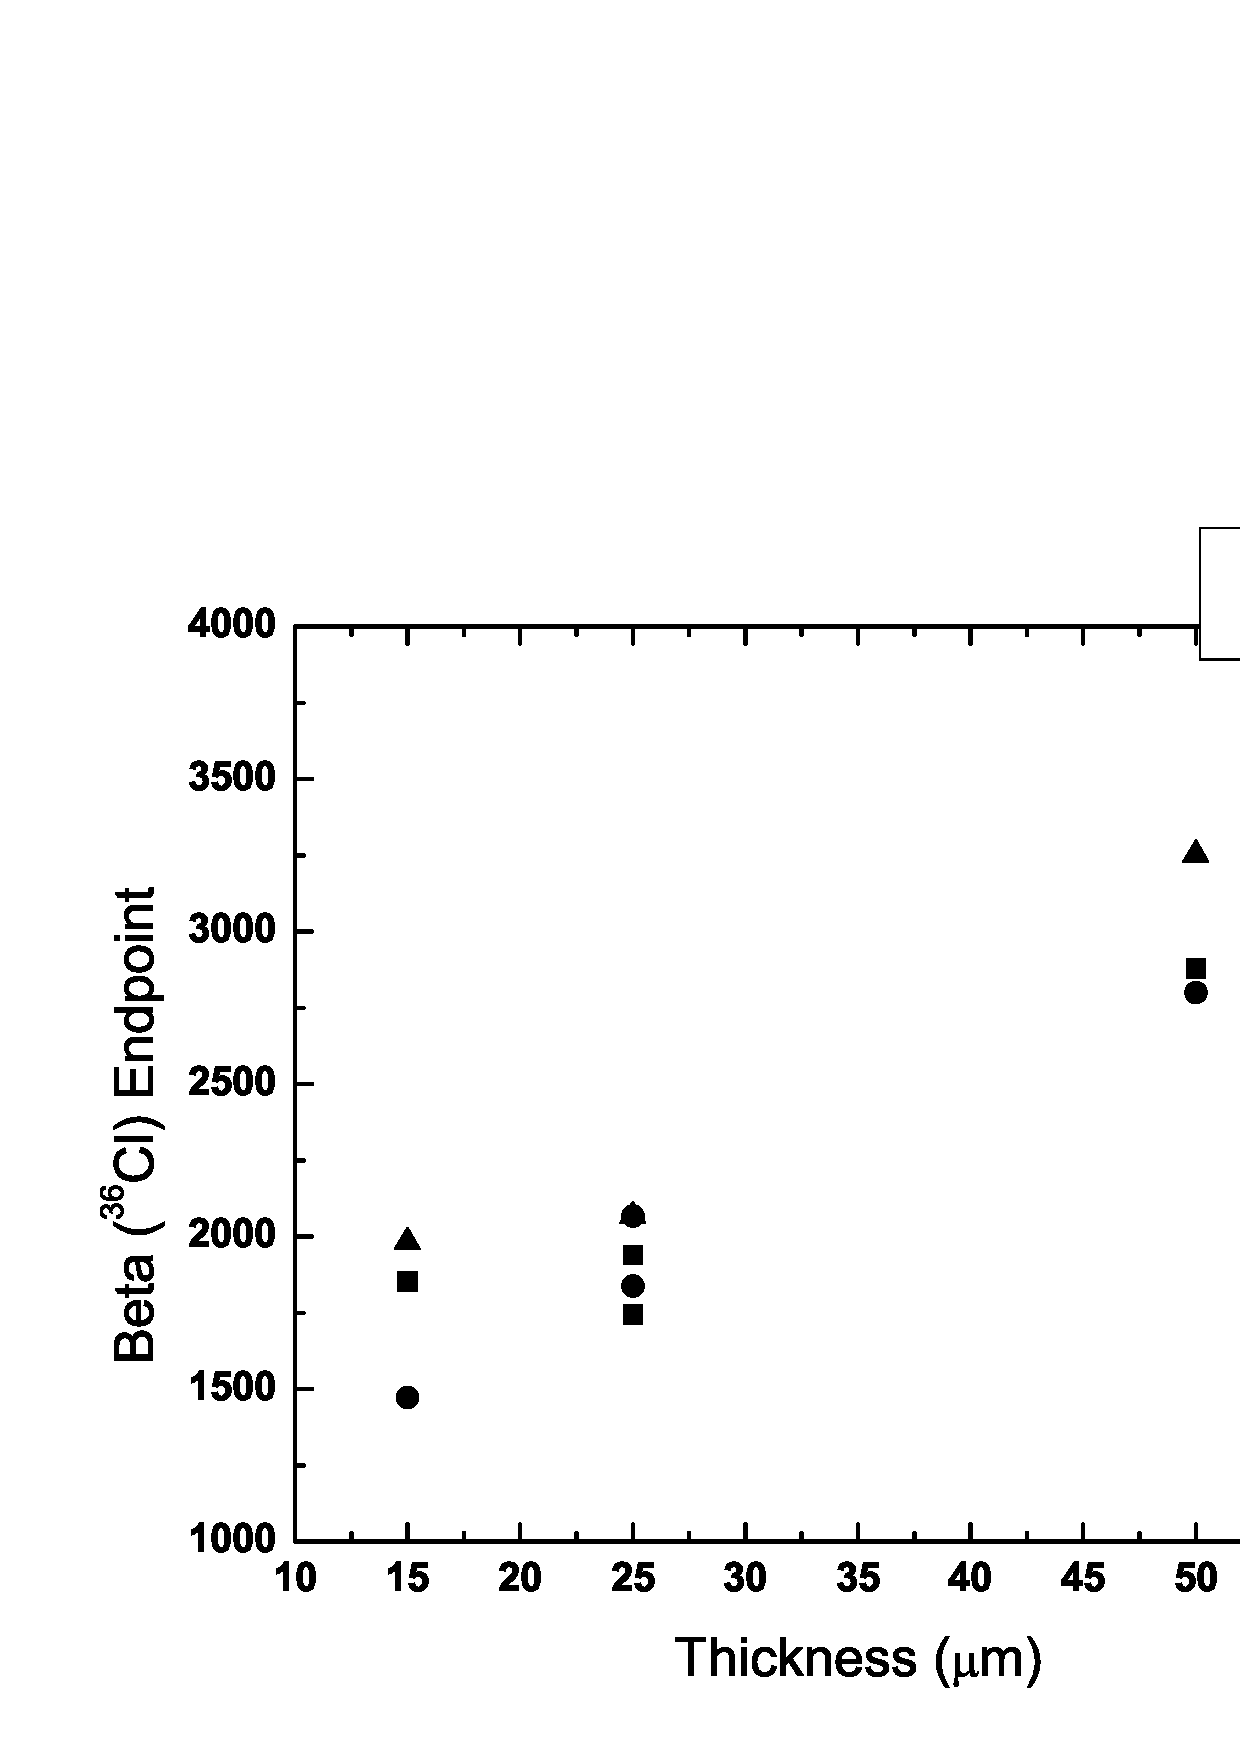
\includegraphics[width=\textwidth]{Beta}
        \caption{Beta Spectra Endpoints for a 5\% PS film}
    \end{subfigure}
    \begin{subfigure}[b]{0.45\figurewidth}
        \includegraphics[width=\textwidth]{PS-5PPOPOPOP_GammaAvg}
        \caption{Gamma Spectra Averages for PS films}
    \end{subfigure}
    \label{fig:SpectraFeatures}
\end{figure}
Figure \ref{fig:GammaIntrNeutronCounts} shows the intrinsic efficiency of these film (from spectra obtained from a \iso{Co}{60} source).
As the film thickness increases the pulse height discriminator at which an intrinsic efficiency of one in a million ($\epsilon_{int,\gamma} \le 10^{-6}$) is reached also increase.
The neutron spectra (shown in the solid lines) does not increase in light yield with increasing thickness, further providing an indication that the thickness of the films can be optimized to maximize the neutron count rates\footnote{The neutron count rate is increased with thickness by the increased mass of the detector} while minimizing the response of the detector to photons.
%%%%%%%%%%%%%%%%%%%% Figures %%%%%%%%%%%%%%%%%%%%%%%%
\begin{figure}
    \centering
    \caption{Gamma intrinsic efficiency (dashed lines) plotted against neutron counts (solid)}
    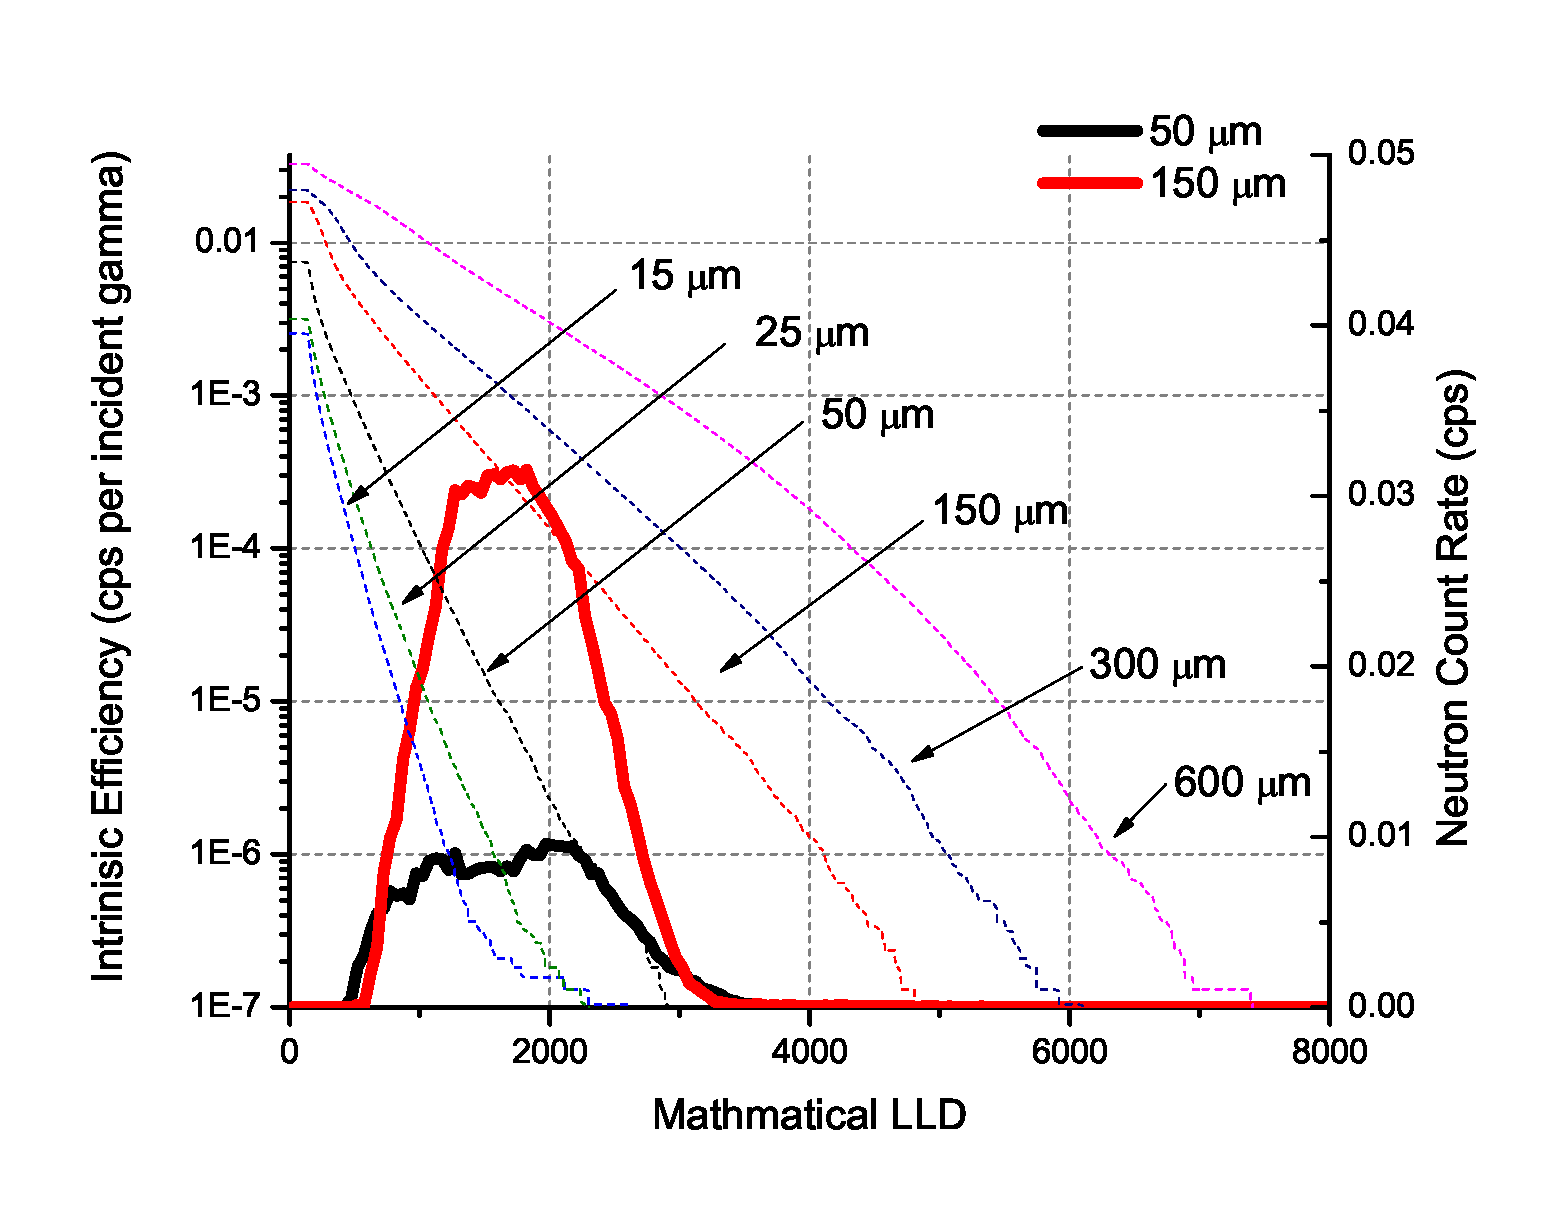
\includegraphics[width=\textwidth]{PS_IntEff_LiF20_PPO5}
    \label{fig:GammaIntrNeutronCounts}
\end{figure}


%%%%%%%%%%%%%%%%%%%%%%%%%%%%%%%%%%%%%
\section{Methods}
\label{sec:Methods}

For convince a subversion repository was created to manage the developed code base, and all source code is available by anonymous checkout from \verb+http://www.murphs-code-repository.googlecode.com/svn/trunk/layeredPolymerTracking+. Revision 360 was the code base used to generate the results shown in \ref{sec:Results}.

\subsubsection{Detector Geometry}
The geometry was setup such that it is possible to define multiple layers of detectors, as shown in Figure \ref{fig:LayerDetectorGeo}.
This was done by creating a 
\begin{figure} 
    \includegraphics[width=\figurewidth]{10LayerGamma}
	\caption{10 Layer Detector with a simulated gamma event}
    \label{fig:LayerDetectorGeo}
\end{figure}
\subsubsection{Physics Lists}

\section{Results}
\label{sec:Results}

\subsection{Parmater Search}

The parameter search for the optimal C and $\sigma$ parameters is shown in the contour plots of Figures \ref{fig:ParamLiver}, \ref{fig:ParamGlass} and \ref{fig:ParamGlass}.
The optimal classifier parameters are shown for the coarse parameter search in Table \ref{tab:CoarseParamValues} and for the fine parameter search in Table \ref{tab:FineParamValues}.
\todo{Make some quantifications and discuss the data}
\begin{table}[h!]
\caption{Coarse Optimal Classifier Parameters}
\label{tab:CoarseParamValues}
\begin{tabular}{c c c c c c c c}
\hline
Data Set & $C_{min}$ & $C_{max}$ & $\sigma_{min}$ & $\sigma_{max}$ & $C$ & $\sigma$ & $\epsilon$ \\ 
\hline
Glass & -5.00 & 5.00 & -5.00 & 5.00 & 5.00 & 0.56 & 72.78 \\ 
Liver & -5.00 & 5.00 & -5.00 & 5.00 & 3.89 & -2.78 & 74.33 \\ 
Vowel & -5.00 & 5.00 & -5.00 & 5.00 & 5.00 & 2.78 & 99.24 \\ 
\hline
\end{tabular}
\end{table}
\begin{table}[ht]
\caption{Fine Optimal Classifier Parameters}
\label{tab:FineParamValues}
\begin{tabular}{c c c c c c c c}
Data Set & $C_{min}$ & $C_{max}$ & $\sigma_{min}$ & $\sigma_{max}$ & $C$ & $\sigma$ & $\epsilon$ \\ 
\hline
Glass & 2.50 & 7.50 & 0.28 & 0.83 & 6.71 & 0.31 & 75.00 \\ 
Liver & 1.94 & 5.83 & -4.17 & -1.39 & 3.79 & -1.68 & 75.67 \\ 
Vowel & 2.50 & 7.50 & 1.39 & 4.17 & 7.50 & 1.97 & 99.43 \\ 
\hline
\end{tabular}
\end{table}
\begin{figure*}[ht!]
	\centering
	\begin{subfigure}[b]{0.45\textwidth}
		\centering
		\includegraphics[width=\textwidth]{Liver_coarseSearch}
        \caption{Coarse Search}
	\end{subfigure}%
	~
	\begin{subfigure}[b]{0.45\textwidth}
		\centering
		\includegraphics[width=\textwidth]{Liver_fineSearch}
        \caption{Fine Search}
	\end{subfigure}	
	\caption{Parameter search for Liver Disorder}
	\label{fig:ParamLiver}

	\begin{subfigure}[b]{0.45\textwidth}
		\centering
		\includegraphics[width=\textwidth]{Glass_coarseSearch}
        \caption{Coarse Search}
	\end{subfigure}%
	~
	\begin{subfigure}[b]{0.45\textwidth}
		\centering
		\includegraphics[width=\textwidth]{Glass_fineSearch}
        \caption{Fine Search}
	\end{subfigure}	
	\caption{Parameter search for Glass Disorder}
	\label{fig:ParamGlass}

	\begin{subfigure}[b]{0.45\textwidth}
		\centering
		\includegraphics[width=\textwidth]{Vowel_coarseSearch}
        \caption{Coarse Search}
	\end{subfigure}%
	~
	\begin{subfigure}[b]{0.45\textwidth}
		\centering
		\includegraphics[width=\textwidth]{Vowel_fineSearch}
        \caption{Fine Search}
	\end{subfigure}	
	\caption{Parameter search for Vowel Disorder}
	\label{fig:ParamVowel}
\end{figure*}

\subsection{AdaBoostM1}

\end{document}

